\documentclass{article}
\usepackage[margin=1in]{geometry}
\usepackage{amsmath,amsthm,amssymb}
\usepackage{bbm,enumerate,mathtools}
\usepackage{tikz,pgfplots}
\usepackage{chessboard}
\usepackage[hidelinks]{hyperref}
\usepackage{multicol} % Problem 35
\usepackage{xstring} % Difficulty command
\usetikzlibrary{shapes.geometric}

\newenvironment{question}{\begin{trivlist}\item[\textbf{Question.}]}{\end{trivlist}}
\newenvironment{note}{\begin{trivlist}\item[\textbf{Note.}]}{\end{trivlist}}
\newenvironment{references}{\begin{trivlist}\item[\textbf{References.}]}{\end{trivlist}}
\newenvironment{related}{\begin{trivlist}\item[\textbf{Related.}]\end{trivlist}\begin{enumerate}}{\end{enumerate}}

\newcommand\score[1]{
\pgfmathsetmacro\pgfxa{#1+1}
\tikzstyle{scorestars}=[
  star,
  star points=5,
  star point ratio=2.25,
  draw,
  inner sep=3pt,
  anchor=outer point 5
]
  \begin{tikzpicture}[baseline]
    \draw[opacity=0] (0,-0.5) rectangle (0,0.2); % Workaround for whitespace at the bottom.
    \foreach \i in {1,...,4} {
      \pgfmathparse{(\i<=#1?"yellow":"gray")}
      \edef\starcolor{\pgfmathresult}
      \draw (\i*4.5ex,0) node[name=star\i,scorestars,fill=\starcolor]  {};
    }
  \end{tikzpicture}
}

\newcommand{\difficulty}[1]{%
  \IfEqCase{#1}{%
      {1}{
        
\begin{tikzpicture}[scale=0.7, baseline=0.9mm]%
          \definecolor{slopegreen}{rgb}{0.0, 0.5, 0.0}%
          \fill[slopegreen] (0.5,0.5) circle (0.5);%
        \end{tikzpicture}%
      }%
      {2}{
        
\begin{tikzpicture}[scale=0.7, baseline=0.9mm]%
          \definecolor{slopeblue}{rgb}{0.0, 0.44, 1.00}
          \fill[slopeblue] (0,0) rectangle (1,1);%
        \end{tikzpicture}%
      }%
      {3}{
\begin{tikzpicture}[scale=0.7, baseline=0.9mm]\fill (0,0.5)--(0.5, 0)--(1,0.5)--(0.5,1)--cycle; \end{tikzpicture}}%
      {4}{
\begin{tikzpicture}[scale=0.7, baseline=0.9mm]\fill (0.25,0)--(0,0.5)--(0.25,1)--(0.5,0.5)--cycle; \fill (0.75,0)--(0.5,0.5)--(0.75,1)--(1,0.5)--cycle;\end{tikzpicture}}%
      % you can add more cases here as desired
  }[\PackageError{difficulty}{Undefined difficulty level: #1}{}]%
}%
\newcommand{\rating}[2]{\difficulty{#1}\\\score{#2}\\}


\begin{document}

\rating{3}{1}
The Snake Cube is \begin{quote}
  a mechanical puzzle, a chain of $27$ or $64$ cubelets, connected by an elastic
  band running through them. The cubelets can rotate freely. The aim of the
  puzzle is to arrange the chain in such a way that they will form
  $3 \times 3 \times 3$ or $4 \times 4 \times 4$ cube.
\end{quote}

\begin{figure}[ht!]
  \centering
  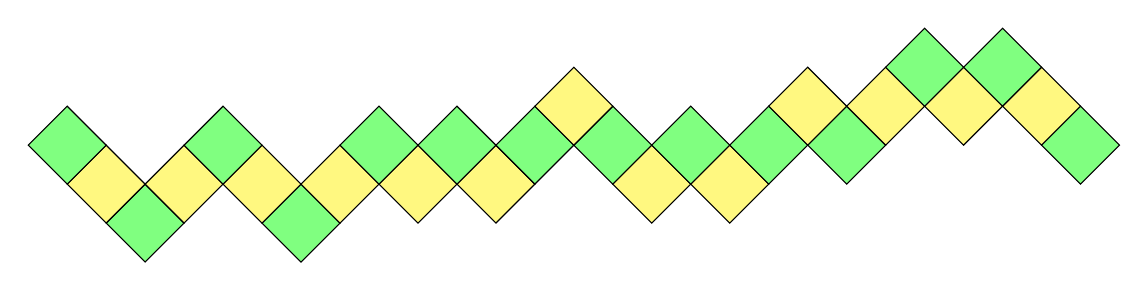
\begin{tikzpicture}[rotate=135,scale=0.7]
    \foreach \x/\y/\c in {
      11/13/green,12/13/yellow,13/13/green,
      11/12/yellow,
      9/11/green,10/11/yellow,11/11/green,
      9/10/yellow,
      8/9/yellow, 9/9/green,
      7/8/yellow, 8/8/green,
      7/7/green,
      5/6/yellow, 6/6/green, 7/6/yellow,
      4/5/yellow, 5/5/green,
      4/4/green,
      3/3/green, 4/3/yellow,
      3/2/yellow,
      2/1/yellow, 3/1/green,
      0/0/green, 1/0/yellow, 2/0/green}
    {
      \fill[\c!50, draw={black}] (\x, \y) rectangle (\x + 1, \y + 1);
    }
  \end{tikzpicture}
  \caption{The most common instance of the Snake Cube.}
\end{figure}

\begin{question}
  How many chains exists for an $n \times n \times n$ cube?
\end{question}

\begin{related}
  \item How about for an $n \times m \times p$ rectangular prism?
  \item Can the ``hardest'' puzzles be quantified? Perhaps those with the
  greatest or fewest number of solutions?
  \item Can this be generalized to higher dimensions?
  \item Can this be generalized to other polytopes?
\end{related}

\begin{references}
  \item Problem 48.
  \item Problem 101.
  \item \url{https://en.wikipedia.org/wiki/Snake_cube}
  \item \url{https://github.com/scholtes/snek} (Counts solutions to \href{https://en.wikipedia.org/wiki/Rubik%27s_Snake}{Rubik's Snake})
\end{references}
\end{document}
